%建议使用pdfLaTeX编译
\documentclass[12pt,a4paper,UTF8]{article}
\bibliographystyle{plain}
\usepackage{geometry}   %页边距调整
\geometry{left=2.0cm,right=2.0cm,top=2.5cm,bottom=2.5cm}
\usepackage{CJKutf8}   %中文输入
\usepackage[hyperref, UTF8]{ctex}   %中文目录标题、章节编号、参考文献标题
\hypersetup{colorlinks=true, linkcolor=black, filecolor=blue, urlcolor=blue, citecolor=blue}   %取消目录的默认红框显示
\usepackage{makeidx}
\usepackage{pgf}   %创建PostScript和pdf格式的图形
\usepackage{tikz}   %配合pgf宏包创建复杂图表,例如函数图像
\usetikzlibrary{math}   %tikz宏包中的库,用于在画图时自己创建变量
\usepackage{extpfeil}   %extpfeil扩展添加了更多用于生成可扩展箭头的宏,例如\xlongequal等
\usepackage{txfonts}   %数学字符库
\usepackage{amsmath}   %更好的数学排版环境,里面提供了更多函数,例如\text{}、\operatorname{}等
\usepackage{latexsym}   %使用不同的符号字体宏包
\usepackage{longtable}   %可换页表格
\usepackage{graphicx}   %可导入和调整外部图片
\usepackage{enumerate}   %自定义编号标签
\usepackage{indentfirst}   %可调整首行缩进

\begin{document}
\title{生成模型笔记}
\author{衔瑜\thanks{Email: fish233yeah@163.com}}
\date{\today}
\maketitle

\setlength{\parindent}{2em}   %设置首行缩进为2字符


\section{概率生成模型}
\subsection{概率生成模型基本思想}
\indent 我们可以将我们的训练集看作是对某个高维空间$\Omega$中的一个随机向量$X$进行多次采样得到的结果,这个随机向量服从一个未知的概率分布$P_r$。那么我们可以通过$X$的样本集(即训练集)来学习获得一个参数化模型$P_\theta$,此时学习获得的模型$P_\theta$应当与$P_r$是近似的,之后通过学习到的模型$P_\theta$再进行采样,则就能获得与训练集近似分布的生成结果,这便是生成网络的基本思想。\\
\indent 然而在实际操作中,由于待拟合的概率分布$p_r$往往非常复杂,神经网络通常很难直接拟合,且另一方面生成的结果很难量化评估其好坏,因此并不能简单地去构造一个生成网络来解决问题。

\subsection{交叉熵}
\subsubsection{定义}
\indent 对于分布为 $p\left(X\right)$ 的随机变量 $X$,我们用概率分布为 $q$ 的编码对真实分布为 $p$ 的信息 $X$ 进行编码的长度我们就称为交叉熵,其表达式为
\[H\left(p,q\right)=E_{x\sim p\left(X\right)}\left[-\log q\left(X\right)\right]=\left\{
\begin{matrix}
-\sum\limits_{x\in X}\left[p\left(x\right)\log q\left(x\right)\right]&,&x\sim p\left(X\right)\text{为离散概率分布}\\
-\int\limits_{x\in X}p\left(x\right)\log q\left(x\right)dx&,&x\sim p\left(X\right)\text{为连续概率分布}\\
\end{matrix}
\right.\]
在给定 $p$ 的情况下,$q$ 和 $p$ 越接近,则交叉熵越小;反之则越大。

\subsection{KL散度}
\subsubsection{定义}
\indent KL散度(Kullback-Leibler Divergence)在概率模型中一般用于度量两个概率密度函数之间的“距离”,其定义为
\[KL\left[p\left(X\right)||q\left(X\right)\right]=E_{x\sim p\left(X\right)}\left[\log\left(\frac{p\left(X\right)}{q\left(X\right)}\right)\right]=\left\{
\begin{matrix}
\sum\limits_{x\in X}\left[p\left(x\right)\log\left(\frac{p\left(x\right)}{q\left(x\right)}\right)\right]&,&x\sim p\left(X\right)\text{为离散概率分布}\\
\int\limits_{x\in X}p\left(x\right)\log\left(\frac{p\left(x\right)}{q\left(x\right)}\right)dx&,&x\sim p\left(X\right)\text{为连续概率分布}\\
\end{matrix}
\right.\]
可以证明KL散度必然大于等于0。注意到KL散度的定义中 $KL\left[p\left(X\right)||q\left(X\right)\right]$ 关于 $p\left(X\right)$、 $q\left(X\right)$ 并不对称,即 $KL\left[p\left(X\right)||q\left(X\right)\right]\neq KL\left[q\left(X\right)||p\left(X\right)\right]$,因此KL散度不满足对称性,显然不是数学意义上的“度量”。\\
\indent 在优化问题中,常用 $p\left(X\right)$ 表示真实分布, $q\left(X\right)$ 表示一个用于拟合 $p\left(X\right)$ 的近似分布,在这种情形下,通常称 $KL\left[p\left(X\right)||q\left(X\right)\right]$ 为前向KL散度(forward Kullback-Leibler Divergence),而称 $KL\left[q\left(X\right)||p\left(X\right)\right]$ 为反向KL散度(reverse Kullback-Leibler Divergence)。

\subsubsection{两类KL散度拟合效果定性分析}
\begin{enumerate}
\item 极小化前向KL散度代价下的拟合行为特性:寻找均值\\
前向KL的计算式中, $p\left(X\right)$ 和 $q\left(X\right)$ 在每个样本点 $x$ 上的差异程度被 $p\left(X\right)$ 加权平均,我们基于此对前向KL的特性进行分析。\\
考虑随机变量 $X$ 的子集 $X_0=\left\{x|p\left(x\right)=0\right\}$,由于 $p\left(X\right)$ 是前向KL公式中的权重系数,因此 $X_0$ 中的元素实际上对前向KL的值没有任何影响。换言之,对任意 $x\in X_0$,无论 $p\left(X_0\right)$ 与 $q\left(X_0\right)$ 相差多大都对前向KL的计算结果毫无影响,因此前向KL值不受 $q\left(X\right)$ 在子集 $X_0=\left\{x|p\left(x\right)=0\right\}$ 上取值的影响。在极小化前向KL散度的过程中,每当 $p\left(X\right)=0$ 时, $q\left(X\right)$ 就会被无视。从连续性角度推理,最小化前向KL散度倾向于忽视“ $q\left(X\right)$ 在满足 $p\left(X\right)$ 近似为0的随机变量取值集合上的拟合精度”,而去更努力的实现“ $q\left(X\right)$ 在满足 $p\left(X\right)>0$ 的随机变量取值集合上的拟合精度”。最小化前向KL散度代价在等价于对 $q\left(X\right)$ 中的参数 $\theta$ 的极大似然估计\\
\indent 前向KL散度的这种特性一般也被称为zero avoiding,原因是它倾向于避免在任何 $p\left(X\right)>0$ 的位置 $x$ 使得 $q\left(X\right)=0$。图\ref{kl_img}左展示了使用前向KL散度代价拟合一个多峰(实际上是双峰)分布的效果示意图
\item 极小化反向KL散度代价下的拟合行为特性:搜寻模态\\
在反向KL中,差异加权求和时的权重系数是 $q\left(X\right)$。此时, $p\left(X\right)$ 在子集 $X_0=\left\{x|q\left(x\right)=0\right\}$ 的取值不影响反向KL值的计算,而当 $q\left(X\right)>0$ 时, $q\left(X\right)$ 与 $p\left(X\right)$ 的差异需要尽可能小以使得反向KL值尽可能小。因此,在以反向KL散度为代价的优化过程中, $q\left(X\right)$ 会更加趋向于要么取值接近0,要么去尽可能贴合 $p\left(X\right)$,表现即为 $q\left(X\right)$ 在拟合 $p\left(X\right)$ 时尽可能保持单一模态。\\
图\ref{kl_img}右展示了使用反向KL散度代价拟合一个多峰(实际上是双峰)分布的效果示意图

\begin{figure}[htb]\centering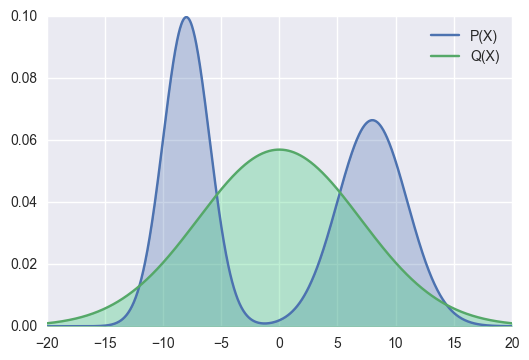
\includegraphics[scale=0.6]{./figure/1.png}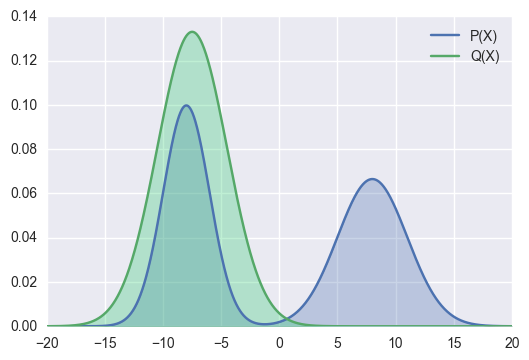
\includegraphics[scale=0.6]{./figure/2.png}\caption{左:前向KL代价拟合;右:反向KL代价拟合}\label{kl_img}\end{figure}

\end{enumerate}

\subsection{VAE (Variational Autoencoders)}

\begin{figure}[htb]\centering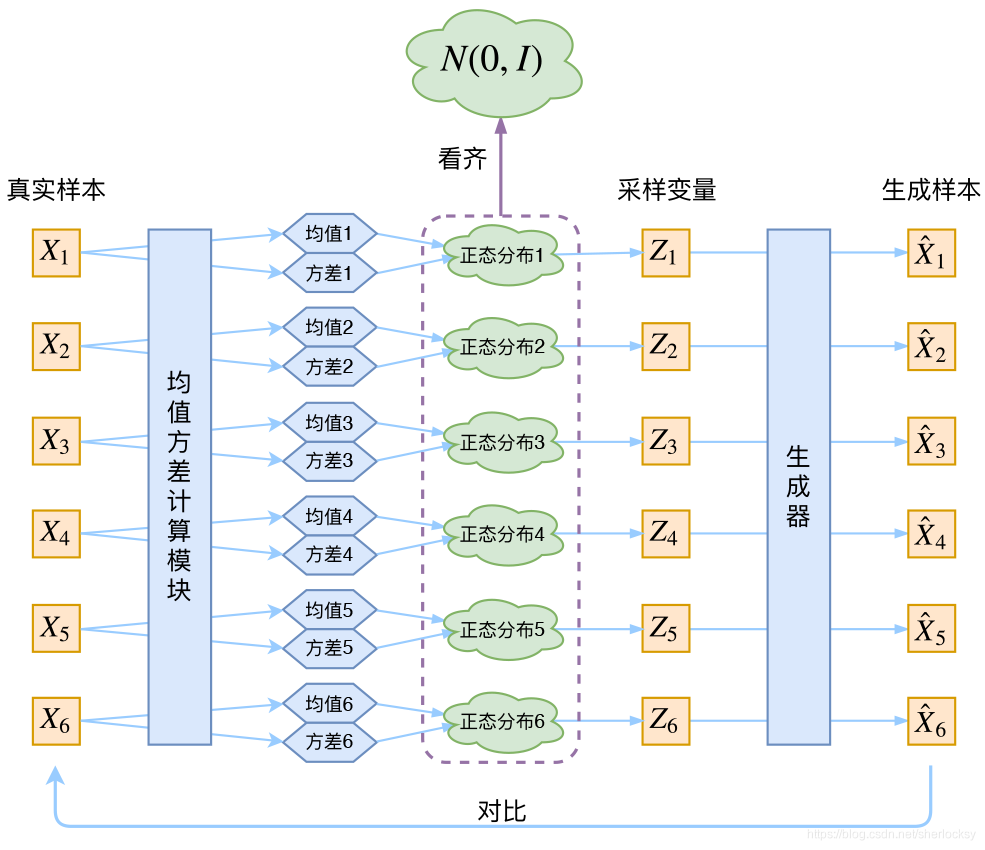
\includegraphics[scale=0.36]{./figure/3.png}\caption{VAE网络结构}\label{vae_img}\end{figure}

\indent VAE整体可以看作encoder-decoder架构。对于一个输入的向量 $x$,它通常包含了许多冗余信息,我们要还原生成这个向量 $x$ 实际上更需要的是描述其本质信息的隐变量 $z$,因此使用了encoder-decoder架构来设计网络,用encoder来进行 $x\to z$ 的编码过程,而decoder则用于 $z\to x$ 的生成过程。\\

\begin{figure}[htb]\centering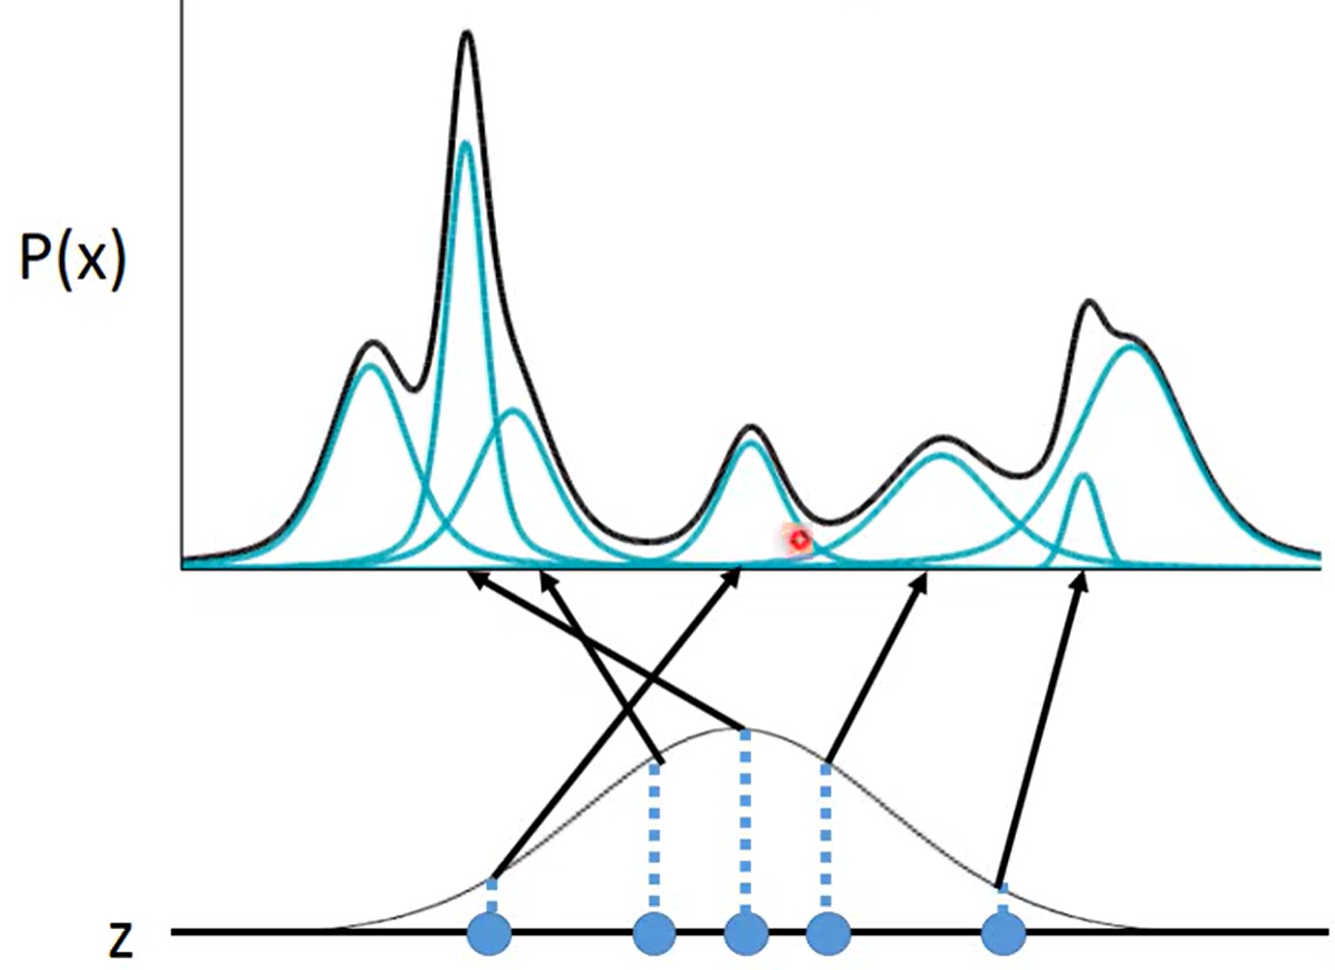
\includegraphics[scale=0.5]{./figure/4.png}\caption{$Z$各点生成高斯分布叠加拟合$P\left(X\right)$}\label{dmm_img}\end{figure}

\indent 首先考虑以下网络的decoder,即生成部分。如图\ref{dmm_img}所示,由于目标概率密度函数 $p_r\left(X\right)$ 通常并不是一个上凸函数,它通常会具有多个极值,所以我们可以考虑使用多个高斯分布相叠加去拟合概率密度函数 $p_r\left(X\right)$,这个思想就是高斯混合模型的思想。我们将隐变量 $Z$ 看作一个随机变量,我们对隐变量 $Z$ 的每个可能的取值,都将其放入一个映射来得到一个均值 $\mu\left(z\right)$ 和一个标准差 $\sigma\left(z\right)$,此时我们便可以从这个隐变量的每个取值分别获得一个高斯分布 $N\left(\mu\left(z\right),\sigma^2\left(z\right)\right)$。因此,如果我们假设 $Z$ 服从某个概率分布,那么对于概率密度函数 $p\left(X\right)$,我们有
\[p\left(x\right)=\int_zp\left(z\right)p\left(x|z\right)dz\]
其中 $p\left(X|Z\right)$ 服从高斯分布 $X|Z\sim N\left(\mu\left(Z\right),\sigma^2\left(Z\right)\right)$,这个 $p\left(X|Z\right)$ 便是 $z\to x$ 的结构,即VAE中的decoder结构。如果我们将 $Z$ 的概率分布确定下来为某个已知分布,那么概率密度函数 $p\left(X\right)$ 就仅与映射 $\mu$ 和 $\sigma$ 相关了。在VAE中我们假设 $Z$ 的概率分布为 $Z\sim N\left(0,1\right)$。\\
\indent 现在再来尝试推导出网络的encoder结构。由于我们的目标是在训练集上最大化 $\sum\limits_x\log p\left(x\right)$,我们假设 $Z|X$ 上有一个任意的概率密度函数 $q\left(Z|X\right)$,对 $\log p\left(X\right)$ 做变换我们有:
\[\begin{aligned}
\log p\left(x\right)&=\log p\left(x\right)\cdot\int_zq\left(z|x\right)dz\\
&=\int_zq\left(z|x\right)\log p\left(x\right)dz\\
&=\int_zq\left(z|x\right)\log\left(\frac{p\left(z,x\right)}{p\left(z|x\right)}\right)dz\\
&=\int_zq\left(z|x\right)\log\left(\frac{p\left(z,x\right)}{q\left(z|x\right)}\cdot\frac{q\left(z|x\right)}{p\left(z|x\right)}\right)dz\\
&=\int_zq\left(z|x\right)\log\left(\frac{p\left(z,x\right)}{q\left(z|x\right)}\right)dz+\int_zq\left(z|x\right)\log\left(\frac{q\left(z|x\right)}{p\left(z|x\right)}\right)dz\\
&=\int_zq\left(z|x\right)\log\left(\frac{p\left(x|z\right)p\left(z\right)}{q\left(z|x\right)}\right)dz+KL\left[q\left(z|x\right)||p\left(z|x\right)\right]\\
\end{aligned}\]
我们记 $L_b=\int_zq\left(z|x\right)\log\left(\frac{p\left(x|z\right)p\left(z\right)}{q\left(z|x\right)}\right)dz$,则我们便得到了如下式子
\[\log p\left(x\right)=L_b+KL\left[q\left(z|x\right)||p\left(z|x\right)\right]\geq L_b\]
此时很直观地,我们似乎只要调整 $p\left(x|z\right)$ 和 $q\left(z|x\right)$ 来将 $L_b$ 最大化即可将 $log p\left(x\right)$ 最大化了,但由于 $p\left(z|x\right)$ 与 $p\left(x|z\right)$ 相关联,在调整 $p\left(x|z\right)$ 的时候可能会导致 $KL\left[q\left(z|x\right)||p\left(z|x\right)\right]$ 下降从而导致 $log p\left(x\right)$ 反而下降,而由于 $q\left(z|x\right)$ 为任意概率密度函数,它变化时并不会导致 $p$ 变化,因此我们考虑先把 $p\left(x|z\right)$ 固定(此时 $\log p\left(x\right)=\log\left(\int_zp\left(z\right)p\left(x|z\right)dz\right)$ 也会固定),仅调整 $q\left(z|x\right)$。显然,当 $q\left(z|x\right)$ 逼近 $p\left(z|x\right)$ 时, $KL\left[q\left(z|x\right)||p\left(z|x\right)\right]$ 会趋近于0,此时 $\log p\left(x\right)$ 会趋近于 $L_b$,因此,在将 $q\left(z|x\right)$ 逼近 $p\left(z|x\right)$ 的情况下再通过调整 $p\left(z|x\right)$ 来增大 $L_b$ 时, $\log p\left(x\right)$ 也会随之增大。而对于 $L_b$,我们有
\[\begin{aligned}
L_b&=\int_zq\left(z|x\right)\log\left(\frac{p\left(x|z\right)p\left(z\right)}{q\left(z|x\right)}\right)dz\\
&=\int_zq\left(z|x\right)\log p\left(x|z\right)dz+\int_zq\left(z|x\right)\log\left(\frac{p\left(z\right)}{q\left(z|x\right)}\right)dz\\
&=E_{Z\sim q\left(z|x\right)}\left[\log p\left(x|z\right)\right]-KL\left[q\left(z|x\right)||p\left(z\right)\right]\\
\end{aligned}\]
此时我们便得到了我们最终所需的表达式:
\[\log p\left(x\right)=E_{Z\sim q\left(z|x\right)}\left[\log p\left(x|z\right)\right]-KL\left[q\left(z|x\right)||p\left(z\right)\right]+KL\left[q\left(z|x\right)||p\left(z|x\right)\right]\]
我们来逐个解析表达式中的三项内容:

\begin{enumerate}
\item $KL\left[q\left(z|x\right)||p\left(z|x\right)\right]$\\
在上文我们已经讲述过,我们要最大化 $\log p\left(x\right)$ 就会希望极小化 $KL\left[q\left(z|x\right)||p\left(z|x\right)\right]$,这便意味着我们希望使用 $q\left(z|x\right)$ 去逼近 $p\left(z|x\right)$,即使用 $q\left(z|x\right)$ 来作为网络的encoder部分
\item $KL\left[q\left(z|x\right)||p\left(z\right)\right]$\\
要最大化 $\log p\left(x\right)$,则 $KL\left[q\left(z|x\right)||p\left(z\right)\right]$ 就需要尽可能的小,而这项KL散度的直观含义也很显然,即我们希望 $x\to z$ 的过程产生的 $Z$ 的分布 $q\left(z|x\right)$ 尽可能与我们假设的 $Z$ 的分布 $p\left(z\right)$ 近似,因此encoder部分还需要满足其概率分布为预先假设的 $Z$ 的分布
\item $E_{Z\sim q\left(z|x\right)}\left[\log p\left(x|z\right)\right]$\\
最大化 $\log p\left(x\right)$ 显然就会需要最大化期望 $E_{Z\sim q\left(z|x\right)}\left[\log p\left(x|z\right)\right]$,而最大化这项期望的含义也很直观:我们希望在给定encoder输出 $q\left(z|x\right)$ 的情况下,decoder的输出 $p\left(x|z\right)$ 的均值尽可能大。
\end{enumerate}

\indent 现在对照网络结构图\ref{vae2_img},显然 $q\left(z|x\right)$ 对应的即为网络encoder部分,它需要去近似 $Z$ 的分布,而根据我们对 $p\left(z\right)$ 的假设 $q\left(z|x\right)$ 将会趋近于一个标准正态分布,此时对 $q\left(z|x\right)$ 进行采样便可以得到 $z$, 并传入decoder部分。网络的decoder部分则为最开始所说的 $p\left(x|z\right)$,即 $X|Z\sim N\left(\mu\left(Z\right),\sigma^2\left(Z\right)\right)$,用于使用高斯分布的输出去近似数据分布。

\begin{figure}[htb]\centering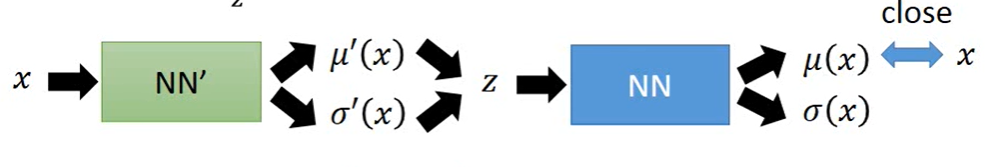
\includegraphics[scale=0.6]{./figure/5.png}\caption{VAE算法结构}\label{vae2_img}\end{figure}

\subsection{DDPM (Denoising Diffusion Probabilistic Models)}
\indent 概率扩散模型的原理与VAE在某些地方有些相似。在DDPM中,我们将通过多次高斯扩散过程 $q\left(x_t|x_{t-1}\right)$ 逐渐将源输入 $X_0$ 转变为随机噪声 $X_T$,再从随机噪声 $X_T$ 学习获得逆扩散过程 $p_\theta\left(x_{t-1}|x_t\right)$ 还原源输入 $X_0$。通过对扩散过程进行学习得到一系列马尔可夫逆扩散过程 $p_\theta\left(x_{t-1}|x_t\right)$ 后,我们便获得了从随机噪声到目标数据的条件分布 $\prod\limits_{t=1}^{T}p_\theta\left(x_{t-1}|x_t\right)$,如图\ref{ddpm_img}所示

\begin{figure}[htb]\centering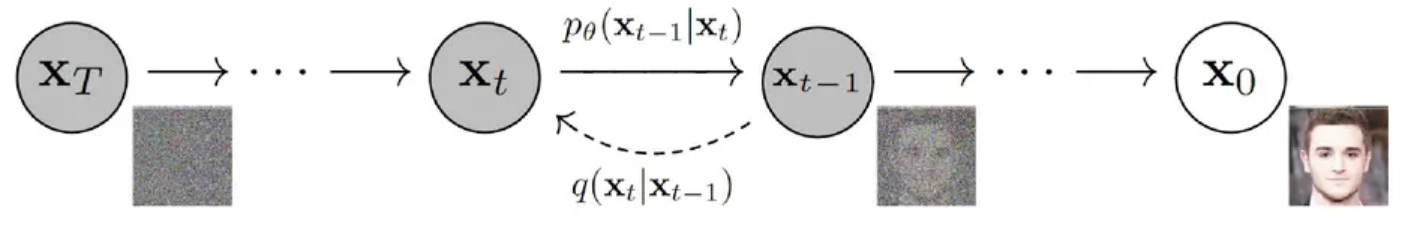
\includegraphics[scale=0.6]{./figure/6.png}\caption{DDPM算法结构}\label{ddpm_img}\end{figure}

\indent 我们先来讨论扩散过程。扩散过程实质上就是多次迭代向数据分布 $X_0\sim q\left(x\right)$ 中添加高斯噪声的一个马尔可夫链过程,这个过程是固定的,且服从分布
\[q\left(X_t|X_{t-1}\right)=N\left(X_t;\sqrt{1-\beta_t}X_{t-1},\beta_tI\right)\qquad q\left(X_{1:T}|X_0\right)=\prod\limits_{t=1}^{T}q\left(X_t|X_{t-1}\right)\]
其中 $\left\{\beta_t\in \left(0,1\right)\right\}_{t=1}^{T}$, $I$ 为单位矩阵。由于这个过程是确定的,因此任意时刻的分布 $q\left(X_t\right)$ 完全可以由 $X_0$ 及 $\beta_1,\beta_2,\cdots,\beta_t$ 确定。对 $X_t|X_{t-1}$,显然我们有
\[\frac{X_t|X_{t-1}-\sqrt{1-\beta_t}X_{t-1}}{\sqrt{\beta_tI}}\sim N\left(0,I\right)\]
设一系列 $\left\{Z\sim N\left(0,I\right)\right\}$ 以及设 $\alpha_t=1-\beta_t,\ \bar{\alpha}_t=\prod\limits_{i=1}^t\alpha_i$,此时我们从上式得到
\[X_t|X_{t-1}=\sqrt{\alpha_t}X_{t-1}+\sqrt{1-\alpha_t}Z_{t-1}\]
将上式中的 $X_{t-1}$ 替换为条件分布 $X_{t-1}|X_{t-2}$,则
\[\begin{aligned}
X_t|X_{t-1}|X_{t-2}&=\sqrt{\alpha_t}\left(X_{t-1}|X_{t-2}\right)+\sqrt{1-\alpha_t}Z_{t-1}\\
X_t|X_{t-1},X_{t-2}&=\sqrt{\alpha_t}\left(\sqrt{\alpha_{t-1}}X_{t-2}+\sqrt{1-\alpha_{t-1}}Z_{t-2}\right)+\sqrt{1-\alpha_t}Z_{t-1}\\
X_t|X_{t-1},X_{t-2}&=\sqrt{\alpha_t\alpha_{t-1}}X_{t-2}+\sqrt{\alpha_t-\alpha_t\alpha_{t-1}}Z_{t-2}+\sqrt{1-\alpha_t}Z_{t-1}\\
X_t|X_{t-1},X_{t-2}&=\sqrt{\alpha_t\alpha_{t-1}}X_{t-2}+\sqrt{1-\alpha_t\alpha_{t-1}}Z_{t-1,t-2}\\
\end{aligned}\]
以此类推,最终我们可以得到
\[X_t|X_{t-1},\cdots,X_0=\sqrt{\bar{\alpha}_t}X_0+\sqrt{1-\bar{\alpha}_t}Z_{t-1,t-2,\cdots,0}\]
即我们有
\[q\left(X_t|X_{0:\left(t-1\right)}\right)=N\left(X_t;\sqrt{\bar{\alpha}_t}X_0,\left(1-\bar{\alpha}_t\right)I\right)\]
由于 $N\left(X_t;\sqrt{\bar{\alpha}_t}X_0,\left(1-\bar{\alpha}_t\right)I\right)$ 仅与 $X_0$ 有关,因此我们有
\[q\left(X_t|X_{0}\right)=N\left(X_t;\sqrt{\bar{\alpha}_t}X_0,\left(1-\bar{\alpha}_t\right)I\right)\]
且有
\[q\left(X_t|X_{t-1}\right)=q\left(X_t|X_{0:\left(t-1\right)}\right)=q\left(X_t|X_{0}\right)\]
显然,当 $\bar{\alpha}_t\to0$ 时, $q\left(X_t|X_0\right)$ 趋近于服从标准正态分布。在原文中,作者将 $\left\{\beta_t\right\}_{t=1}^{T}$ 设置为了线性增加的序列,即 $\beta_1<\beta_2<\cdots<\beta_T$。\\
\indent 接下来我们讨论逆扩散过程。第一步我们先推导一个我们后面会需要用到的后验条件分布:
\[\begin{aligned}
q\left(X_{t-1}|X_t,X_0\right)&=\frac{q\left(X_t,X_{t-1},X_0\right)}{q\left(X_t,X_0\right)}\\
&=\frac{q\left(X_t|X_{t-1},X_0\right)q\left(X_{t-1},X_0\right)}{q\left(X_t,X_0\right)}\\
&=q\left(X_t|X_{t-1}\right)\frac{q\left(X_{t-1}|X_0\right)}{q\left(X_t|X_0\right)}\\
&=\frac{1}{\sqrt{2\pi}\cdot\frac{\sigma_{q\left(X_t|X_{t-1}\right)}\sigma_{q\left(X_{t-1}|X_0\right)}}{\sigma_{q\left(X_t|X_0\right)}}}\cdot e^{-\frac{1}{2}\left[\frac{\left(X_t-\sqrt{\alpha_t}X_{t-1}\right)^2}{\beta_t}+\frac{\left(X_{t-1}-\sqrt{\bar{\alpha}_{t-1}}X_0\right)^2}{1-\bar{\alpha}_{t-1}}-\frac{\left(X_t-\sqrt{\bar{\alpha}_t}X_0\right)^2}{1-\bar{\alpha}_t}\right]}\\
&=\frac{1}{\sqrt{2\pi}\cdot\frac{\sigma_{q\left(X_t|X_{t-1}\right)}\sigma_{q\left(X_{t-1}|X_0\right)}}{\sigma_{q\left(X_t|X_0\right)}}}\cdot e^{-\frac{1}{2}\left[\left(\frac{\alpha_t}{\beta_t}+\frac{1}{1-\bar{\alpha}_{t-1}}\right)X_{t-1}^2-\left(\frac{2\sqrt{\alpha_t}}{\beta_t}X_t+\frac{2\sqrt{\bar{\alpha}_{t-1}}}{1-\bar{\alpha}_{t-1}}X_0\right)X_{t-1}+C\left(X_t,X_0\right)\right]}\\
&=\frac{1}{\sqrt{2\pi}\cdot\frac{\sigma_{q\left(X_t|X_{t-1}\right)}\sigma_{q\left(X_{t-1}|X_0\right)}}{\sigma_{q\left(X_t|X_0\right)}}}\cdot e^{-\frac{1}{2}\left[\frac{\left(X_{t-1}-\frac{\frac{\sqrt{\alpha_t}}{\beta_t}X_t+\frac{\sqrt{\bar{\alpha}_{t-1}}}{1-\bar{\alpha}_{t-1}}X_0}{\frac{\alpha_t}{\beta_t}+\frac{1}{1-\bar{\alpha}_{t-1}}}\right)^2}{\frac{1}{\frac{\alpha_t}{\beta_t}+\frac{1}{1-\bar{\alpha}_{t-1}}}}\right]+C^{\prime}\left(X_t,X_0\right)}\\
&=\frac{1}{\sqrt{2\pi}\cdot\frac{\sigma_{q\left(X_t|X_{t-1}\right)}\sigma_{q\left(X_{t-1}|X_0\right)}}{\sigma_{q\left(X_t|X_0\right)}}}e^{C^{\prime}\left(X_t,X_0\right)}\cdot e^{-\frac{1}{2}\left[\frac{\left(X_{t-1}-\left(\frac{\sqrt{\alpha_t}\left(1-\bar{\alpha}_{t-1}\right)}{1-\bar{\alpha}_t}X_t+\frac{\sqrt{\bar{\alpha}_t-1}\cdot\beta_t}{1-\bar{\alpha}_t}X_0\right)\right)^2}{\frac{1-\bar{\alpha}_{t-1}}{1-\bar{\alpha}_t}\beta_t}\right]}\\
&=\frac{1}{\sqrt{2\pi}\cdot\sigma^{\prime}}\cdot e^{-\frac{1}{2}\left[\frac{\left(X_{t-1}-\left(\frac{\sqrt{\alpha_t}\left(1-\bar{\alpha}_{t-1}\right)}{1-\bar{\alpha}_t}X_t+\frac{\sqrt{\bar{\alpha}_t-1}\cdot\beta_t}{1-\bar{\alpha}_t}X_0\right)\right)^2}{\frac{1-\bar{\alpha}_{t-1}}{1-\bar{\alpha}_t}\beta_t}\right]}\\
\end{aligned}\]
其中, $C\left(X_t,X_0\right)$ 和 $C^{\prime}\left(X_t,X_0\right)$ 均为某个仅与 $X_0$ 和 $X_t$ 有关的函数, $\sigma^{\prime}=\frac{\sigma_{q\left(X_t|X_{t-1}\right)}\cdot\sigma_{q\left(X_{t-1}|X_0\right)}}{\sigma_{q\left(X_t|X_0\right)}\cdot e^{C^{\prime}\left(X_t,X_0\right)}}$。显然,对均值为 $\tilde{\mu}_t\left(X_t,X_0\right)=\frac{\sqrt{\alpha_t}\left(1-\bar{\alpha}_{t-1}\right)}{1-\bar{\alpha}_t}X_t+\frac{\sqrt{\bar{\alpha}_t-1}\cdot\beta_t}{1-\bar{\alpha}_t}X_0$,方差为 $\tilde{\beta}_tI=\frac{1-\bar{\alpha}_{t-1}}{1-\bar{\alpha}_t}\beta_t\cdot I$ 的正态分布 $N\left(X_{t-1};\tilde{\mu}_t\left(X_t,X_0\right),\tilde{\beta}_tI\right)$,我们有
\[\frac{q\left(X_{t-1}|X_t,X_0\right)}{f_{N\left(\tilde{\mu}_t\left(X_t,X_0\right),\tilde{\beta}_tI\right)}\left(X_{t-1}\right)}=\frac{\sqrt{\tilde{\beta}_t}}{\sigma^{\prime}}\]
而由于
\[\int q\left(X_{t-1}|X_t,X_0\right)dx=1=\int f_{N\left(\tilde{\mu}_t\left(X_t,X_0\right),\tilde{\beta}_tI\right)}\left(X_{t-1}\right)dx\]
因此显然有 $\sigma^{\prime}=\sqrt{\tilde{\beta}_t}$,即后验分布 $q\left(X_{t-1}|X_t,X_0\right)$ 服从正态分布 $N\left(X_{t-1};\tilde{\mu}_t\left(X_t,X_0\right),\tilde{\beta}_tI\right)$。\\
\indent 现在我们假设逆扩散过程也是一个马尔可夫链过程,且有
\[p_{\theta}\left(X_{0:\left(T-1\right)}|X_T\right)=\prod\limits_{t=1}^{T}p_{\theta}\left(X_{t-1}|X_t\right)\]
那么对于其对数似然函数,我们有
\[\begin{aligned}
-\log p_{\theta}\left(X_0\right)&\leq -\log p_{\theta}\left(X_0\right)+KL\left[q\left(X_{1:T}|X_{0}\right)||p_{\theta}\left(X_{1:T}|X_{0}\right)\right]\\
&=-\log p_{\theta}\left(X_0\right)+E_{x_{1:T}\sim q\left(X_{1:T}|X_{0}\right)}\left[\log\left(\frac{q\left(X_{1:T}|X_{0}\right)}{p_{\theta}\left(X_{1:T}|X_{0}\right)}\right)\right]\\
&=-\log p_{\theta}\left(X_0\right)+E_{x_{1:T}\sim q\left(X_{1:T}|X_{0}\right)}\left[\log\left(\frac{q\left(X_{1:T}|X_{0}\right)}{\frac{p_{\theta}\left(X_{0:T}\right)}{p_{\theta}\left(X_{0}\right)}}\right)\right]\\
&=-\log p_{\theta}\left(X_0\right)+E_{x_{1:T}\sim q\left(X_{1:T}|X_{0}\right)}\left[\log\left(\frac{q\left(X_{1:T}|X_{0}\right)}{p_{\theta}\left(X_{0:T}\right)}\right)\right]+E_{x_{1:T}\sim q\left(X_{1:T}|X_{0}\right)}\left[\log\left(p_{\theta}\left(X_{0}\right)\right)\right]\\
&=E_{x_{1:T}\sim q\left(X_{1:T}|X_{0}\right)}\left[\log\left(\frac{q\left(X_{1:T}|X_{0}\right)}{p_{\theta}\left(X_{0:T}\right)}\right)\right]\\
\end{aligned}\]
将对数似然转换为交叉熵,我们有
\[\begin{aligned}
E_{x\sim q\left(X_{0}\right)}\left[-\log p_{\theta}\left(X_0\right)\right]&\leq E_{x\sim q\left(X_{0}\right)}\left\{E_{x_{1:T}\sim q\left(X_{1:T}|X_{0}\right)}\left[\log\left(\frac{q\left(X_{1:T}|X_{0}\right)}{p_{\theta}\left(X_{0:T}\right)}\right)\right]\right\}\\
&=E_{x\sim q\left(X_{0}\right)}\left\{\int q\left(X_{1:T}|X_{0}\right)\log\left(\frac{q\left(X_{1:T}|X_{0}\right)}{p_{\theta}\left(X_{0:T}\right)}\right)dX_{1:T}\right\}\\
&=\int q\left(X_{0}\right)\int q\left(X_{1:T}|X_{0}\right)\log\left(\frac{q\left(X_{1:T}|X_{0}\right)}{p_{\theta}\left(X_{0:T}\right)}\right)dX_{1:T}dX_{0}\\
&=\int q\left(X_{0:T}\right)\log\left(\frac{q\left(X_{1:T}|X_{0}\right)}{p_{\theta}\left(X_{0:T}\right)}\right)dX_{0:T}\\
&=E_{x_{0:T}\sim q\left(X_{0:T}\right)}\left[\log\left(\frac{q\left(X_{1:T}|X_{0}\right)}{p_{\theta}\left(X_{0:T}\right)}\right)\right]\\
\end{aligned}\]
设 $L_{VLB}=E_{x_{0:T}\sim q\left(X_{0:T}\right)}\left[\log\left(\frac{q\left(X_{1:T}|X_{0}\right)}{p_{\theta}\left(X_{0:T}\right)}\right)\right]$,那么要最小化交叉熵 $E_{x\sim q\left(X_{0}\right)}\left[-\log p_{\theta}\left(X_0\right)\right]$ 可以考虑直接最小化 $L_{VLB}$。继续推导 $L_{VLB}$,我们有
\[\begin{aligned}
L_{VLB}&=E_{x_{0:T}\sim q\left(X_{0:T}\right)}\left[\log\left(\frac{q\left(X_{1:T}|X_{0}\right)}{p_{\theta}\left(X_{0:T}\right)}\right)\right]\\
&=E_{x_{0:T}\sim q\left(X_{0:T}\right)}\left[\log\left(\frac{\prod\limits_{t=1}^{T}q\left(X_t|X_{t-1}\right)}{p_{\theta}\left(X_T\right)\prod\limits_{t=1}^{T}p_{\theta}\left(X_{t-1}|X_t\right)}\right)\right]\\
&=E_{x_{0:T}\sim q\left(X_{0:T}\right)}\left[-\log p_{\theta}\left(X_T\right)+\sum\limits_{t=1}^{T}\log\left(\frac{q\left(X_t|X_{t-1}\right)}{p_{\theta}\left(X_{t-1}|X_t\right)}\right)\right]\\
&=E_{x_{0:T}\sim q\left(X_{0:T}\right)}\left[-\log p_{\theta}\left(X_T\right)+\log\left(\frac{q\left(X_1|X_0\right)}{p_{\theta}\left(X_0|X_1\right)}\right)+\sum\limits_{t=2}^{T}\log\left(\frac{q\left(X_t|X_{t-1},X_0\right)}{p_{\theta}\left(X_{t-1}|X_t\right)}\right)\right]\\
&=E_{x_{0:T}\sim q\left(X_{0:T}\right)}\left[-\log p_{\theta}\left(X_T\right)+\log\left(\frac{q\left(X_1|X_0\right)}{p_{\theta}\left(X_0|X_1\right)}\right)+\sum\limits_{t=2}^{T}\log\left(\frac{q\left(X_t,X_{t-1},X_0\right)}{p_{\theta}\left(X_{t-1}|X_t\right)\cdot q\left(X_{t-1},X_0\right)}\right)\right]\\
&=E_{x_{0:T}\sim q\left(X_{0:T}\right)}\left[-\log p_{\theta}\left(X_T\right)+\log\left(\frac{q\left(X_1|X_0\right)}{p_{\theta}\left(X_0|X_1\right)}\right)+\sum\limits_{t=2}^{T}\log\left(\frac{q\left(X_{t-1}|X_t,X_0\right)\cdot q\left(X_t,X_0\right)}{p_{\theta}\left(X_{t-1}|X_t\right)\cdot q\left(X_{t-1},X_0\right)}\right)\right]\\
&=E_{x_{0:T}\sim q\left(X_{0:T}\right)}\left[-\log p_{\theta}\left(X_T\right)+\log\left(\frac{q\left(X_1|X_0\right)}{p_{\theta}\left(X_0|X_1\right)}\right)+\sum\limits_{t=2}^{T}\log\left(\frac{q\left(X_{t-1}|X_t,X_0\right)}{p_{\theta}\left(X_{t-1}|X_t\right)}\cdot\frac{q\left(X_t|X_0\right)}{q\left(X_{t-1}|X_0\right)}\right)\right]\\
&=E_{x_{0:T}\sim q\left(X_{0:T}\right)}\left[-\log p_{\theta}\left(X_T\right)+\log\left(\frac{q\left(X_1|X_0\right)}{p_{\theta}\left(X_0|X_1\right)}\right)+\sum\limits_{t=2}^{T}\log\left(\frac{q\left(X_{t-1}|X_t,X_0\right)}{p_{\theta}\left(X_{t-1}|X_t\right)}\right)+\sum\limits_{t=2}^{T}\log\left(\frac{q\left(X_t|X_0\right)}{q\left(X_{t-1}|X_0\right)}\right)\right]\\
&=E_{x_{0:T}\sim q\left(X_{0:T}\right)}\left[-\log p_{\theta}\left(X_T\right)+\sum\limits_{t=2}^{T}\log\left(\frac{q\left(X_{t-1}|X_t,X_0\right)}{p_{\theta}\left(X_{t-1}|X_t\right)}\right)+\log\left(\frac{q\left(X_T|X_0\right)}{p_{\theta}\left(X_0|X_1\right)}\right)\right]\\
&=E_{x_{0:T}\sim q\left(X_{0:T}\right)}\left[\log\left(\frac{q\left(X_T|X_0\right)}{p_{\theta}\left(X_T\right)}\right)+\sum\limits_{t=2}^{T}\log\left(\frac{q\left(X_{t-1}|X_t,X_0\right)}{p_{\theta}\left(X_{t-1}|X_t\right)}\right)-\log p_{\theta}\left(X_0|X_1\right)\right]\\
&=E_{x_{0:T}\sim q\left(X_{0:T}\right)}\left[\log\left(\frac{q\left(X_T|X_0\right)}{p_{\theta}\left(X_T\right)}\right)\right]+\sum\limits_{t=2}^{T}E_{x_{0:T}\sim q\left(X_{0:T}\right)}\left[\log\left(\frac{q\left(X_{t-1}|X_t,X_0\right)}{p_{\theta}\left(X_{t-1}|X_t\right)}\right)\right]-\log p_{\theta}\left(X_0|X_1\right)\\
\end{aligned}\]
最后一步的 $E_{x_{0:T}\sim q\left(X_{0:T}\right)}\left[\log\left(\frac{q\left(X_T|X_0\right)}{p_{\theta}\left(X_T\right)}\right)\right]$ 以及 $T-1$ 项 $E_{x_{0:T}\sim q\left(X_{0:T}\right)}\left[\log\left(\frac{q\left(X_{t-1}|X_t,X_0\right)}{p_{\theta}\left(X_{t-1}|X_t\right)}\right)\right]$ 它们并不是KL散度,因此在这里并没有写成KL散度表示形式。记
\[\begin{aligned}
L_T&=E_{x_{0:T}\sim q\left(X_{0:T}\right)}\left[\log\left(\frac{q\left(X_T|X_0\right)}{p_{\theta}\left(X_T\right)}\right)\right]\\
L_{t-1}&=E_{x_{0:T}\sim q\left(X_{0:T}\right)}\left[\log\left(\frac{q\left(X_{t-1}|X_t,X_0\right)}{p_{\theta}\left(X_{t-1}|X_t\right)}\right)\right]\\
L_0&=-\log p_{\theta}\left(X_0|X_1\right)\\
\end{aligned}\]
\indent 由于最后一步的 $E_{x_{0:T}\sim q\left(X_{0:T}\right)}\left[\log\left(\frac{q\left(X_T|X_0\right)}{p_{\theta}\left(X_T\right)}\right)\right]$ 以及 $T-1$ 项 $E_{x_{0:T}\sim q\left(X_{0:T}\right)}\left[\log\left(\frac{q\left(X_{t-1}|X_t,X_0\right)}{p_{\theta}\left(X_{t-1}|X_t\right)}\right)\right]$ 并不是KL散度,因此我们并不能确定其优化下界是否存在,以及存在的话下界为多少,因此在讨论损失函数优化目标之前我们还需要先证明一下各个 $L_i,i=0,1,\cdots,T$ 的值的取值范围。

\begin{enumerate}
\item $L_T$
\[\begin{aligned}
L_T&=E_{x_{0:T}\sim q\left(X_{0:T}\right)}\left[\log\left(\frac{q\left(X_T|X_0\right)}{p_{\theta}\left(X_T\right)}\right)\right]\\
&=E_{x_{0:T}\sim q\left(X_{0:T}\right)}\left[\log\left(\frac{q\left(X_T|X_{0:\left(T-1\right)}\right)}{p_{\theta}\left(X_T\right)}\right)\right]\\
&=E_{x_{0:T}\sim q\left(X_{0:T}\right)}\left[\log\left(\frac{q\left(X_{0:T}\right)}{p_{\theta}\left(X_T\right)}\right)+\log\left(\frac{1}{q\left(X_{0:\left(T-1\right)}\right)}\right)\right]\\
&=KL\left[q\left(X_{0:T}\right)||p_{\theta}\left(X_T\right)\right]+E_{x_{0:T}\sim q\left(X_{0:T}\right)}\left[\log\left(\frac{1}{q\left(X_{0:\left(T-1\right)}\right)}\right)\right]\\
\end{aligned}\]
由于 $KL\left[q\left(X_{0:T}\right)||p_{\theta}\left(X_T\right)\right]$ 和 $E_{x_{0:T}\sim q\left(X_{0:T}\right)}\left[\log\left(\frac{1}{q\left(X_{0:\left(T-1\right)}\right)}\right)\right]$ 均大于等于0,因此 $L_T$ 大于等于0;又由于当 $q\left(X_T|X_0\right)=p_{\theta}\left(X_T\right)$ 时 $L_T$ 等于0,因此 $L_T$ 的优化下界存在且为0。
\item $L_{t-1}$
\[\begin{aligned}
L_{t-1}&=E_{x_{0:T}\sim q\left(X_{0:T}\right)}\left[\log\left(\frac{q\left(X_{t-1}|X_t,X_0\right)}{p_{\theta}\left(X_{t-1}|X_t\right)}\right)\right]\\
&=E_{x_{0:T}\sim q\left(X_{0:T}\right)}\left[\log\left(\frac{q\left(X_{0:T}\right)}{p_{\theta}\left(X_{t-1}|X_t\right)}\right)+\log\left(\frac{q\left(X_{t-1}|X_t,X_0\right)}{q\left(X_{0:T}\right)}\right)\right]\\
&=KL\left[q\left(X_{0:T}\right)||p_{\theta}\left(X_{t-1}|X_t\right)\right]+E_{x_{0:T}\sim q\left(X_{0:T}\right)}\left[\log\left(\frac{q\left(X_t|X_{t-1}\right)q\left(X_{t-1}|X_0\right)}{q\left(X_{0:T}\right)q\left(X_t|X_0\right)}\right)\right]\\
&=KL\left[q\left(X_{0:T}\right)||p_{\theta}\left(X_{t-1}|X_t\right)\right]+E_{x_{0:T}\sim q\left(X_{0:T}\right)}\left[\log\left(\frac{q\left(X_t|X_{0:\left(t-1\right)}\right)q\left(X_{t-1}|X_{0:\left(t-2\right)}\right)}{q\left(X_{0:T}\right)q\left(X_t|X_{0:\left(t-1\right)}\right)}\right)\right]\\
&=KL\left[q\left(X_{0:T}\right)||p_{\theta}\left(X_{t-1}|X_t\right)\right]+E_{x_{0:T}\sim q\left(X_{0:T}\right)}\left[\log\left(\frac{q\left(X_{0:\left(t-1\right)}\right)}{q\left(X_{0:T}\right)q\left(X_{0:\left(t-2\right)}\right)}\right)\right]\\
&=KL\left[q\left(X_{0:T}\right)||p_{\theta}\left(X_{t-1}|X_t\right)\right]+E_{x_{0:T}\sim q\left(X_{0:T}\right)}\left[\log\left(\frac{1}{q\left(X_{t:T}|X_{0:\left(t-1\right)}\right)q\left(X_{0:\left(t-2\right)}\right)}\right)\right]\\
\end{aligned}\]
由于 $KL\left[q\left(X_{0:T}\right)||p_{\theta}\left(X_{t-1}|X_t\right)\right]$ 和 $E_{x_{0:T}\sim q\left(X_{0:T}\right)}\left[\log\left(\frac{1}{q\left(X_{t:T}|X_{0:\left(t-1\right)}\right)q\left(X_{0:\left(t-2\right)}\right)}\right)\right]$ 均大于等于0,因此 $L_{t-1}$ 大于等于0;又由于当 $q\left(X_{t-1}|X_t,X_0\right)=p_{\theta}\left(X_{t-1}|X_t\right)$ 时 $L_{t-1}$ 等于0,因此 $L_{t-1}$ 的优化下界存在且为0。
\item $L_0$\\
显然 $L_0$ 的优化下界存在且为0。
\end{enumerate}

\indent 因此,根据上述推导过程,要最小化 $L_{VLB}$ 我们就需要最小化各个 $L_i,i=0,1,\cdots,T$,且希望模型逆扩散过程的每一步都去拟合对应的扩散过程的反向概率分布,通过对扩散过程的学习来得到逆扩散的分布,即让 $p_{\theta}\left(X_T\right)$ 学习 $q\left(X_T|X_0\right)$,让 $p_{\theta}\left(X_{t-1}|X_t\right)$ 学习 $q\left(X_{t-1}|X_t,X_0\right)$,最后让 $p_{\theta}\left(X_0|X_1\right)$ 逼近1。而又由于我们证明了 $q\left(X_T|X_0\right)$ 近似服从标准正态分布,且每一步 $q\left(X_{t-1}|X_t,X_0\right)$ 均服从正态分布,因此逆扩散过程的每一步也服从正态分布,因此我们可以假设
\[p_{\theta}\left(X_T\right)=N\left(X_T;0,1\right)\qquad p_{\theta}\left(X_{t-1}|X_t\right)=N\left(X_{t-1};\mu_{\theta}\left(X_t,t\right),\Sigma_{\theta}\left(X_t,t\right)\right)\]
来对生成过程进行拟合。至此,网络结构设计和损失函数设计均推导完毕。


\section{分数生成模型}
\subsection{分数生成模型基本思想}



\newpage
\begin{thebibliography}{99}
\bibitem{nndl}\href{https://xpqiu.github.io/}{邱锡鹏}. \href{https://nndl.github.io/}{神经网络与深度学习}. 机械工业出版社. https://nndl.github.io/. 2020
\bibitem{kl}\href{https://www.zhihu.com/people/adv-adj}{工具人66号}. \href{https://zhuanlan.zhihu.com/p/372835186}{进阶详解KL散度}. 知乎. 2022
\bibitem{vae}\href{https://www.youtube.com/c/HungyiLeeNTU}{Hung-yi Lee}. \href{https://www.youtube.com/watch?v=8zomhgKrsmQ&list=PLJV_el3uVTsPy9oCRY30oBPNLCo89yu49&index=27}{ML Lecture 18: Unsupervised Learning - Deep Generative Model (Part II)}. Youtube. 2016
\bibitem{ddpm}\href{https://space.bilibili.com/373596439}{deep\_thoughts}. \href{https://www.bilibili.com/video/BV1b541197HX?vd_source=e1a23aab8211cd62864bd7e4ee217986}{Probabilistic Diffusion Model概率扩散模型理论与完整PyTorch代码详细解读}. bilibili. 2022
\end{thebibliography}


\end{document}
















































